\chapter{Specifikacija programske potpore}
		
	\section{Funkcionalni zahtjevi}
			
			%\textbf{\textit{dio 1. revizije}}\\
			
			%\textit{Navesti \textbf{dionike} koji imaju \textbf{interes u ovom sustavu} ili  \textbf{su nositelji odgovornosti}. To su prije svega korisnici, ali i administratori sustava, naručitelji, razvojni tim.}\\
				
			%\textit{Navesti \textbf{aktore} koji izravno \textbf{koriste} ili \textbf{komuniciraju sa sustavom}. Oni mogu imati inicijatorsku ulogu, tj. započinju određene procese u sustavu ili samo sudioničku ulogu, tj. obavljaju određeni posao. Za svakog aktora navesti funkcionalne zahtjeve koji se na njega odnose.}\\
			
			
			\noindent \textbf{Dionici:}
			 
			\begin{packed_enum}
				
				\item Neregistrirani korisnik
				\item Registrirani korisnik				
				\item Administrator
                \item Trgovina\\
				
			\end{packed_enum}
   
			
			\noindent \textbf{Aktori i njihovi funkcionalni zahtjevi:}
			
			
			\begin{packed_enum}
				\item  \underbar{Neregistrirani korisnik (inicijator) može:}
				
				\begin{enumerate}
					
					\item pregledavati sadržaj aplikacije
					\item se registrirati u sustav, stvoriti novi korisnički račun za koji su mu potrebni korisničko ime, prezime, nadimak i e-mail
			
					
				\end{enumerate}
			
				\item  \underbar{Registrirani korisnik (sudionik) može:}
				
				\begin{enumerate}
					
					\item birati što od navedenog će biti javno, a što privatno
					\item pregledavati sadržaj aplikacije
        	        \item unositi cijene i dodavati oznake proizvodima
                        \item predložiti oznaku za proivod
                        
					
				\end{enumerate}

                \item  \underbar{Administrator (sudionik) može:}
				
				\begin{enumerate}
					
					\item birati što od navedenog će biti javno, a što privatno
					\item pregledavati sadržaj aplikacije
        	        \item unositi cijene i dodavati oznake proizvodima
                        \item zabraniti pristup stranici registriranim korisnicima ili trgovinama
                        \item napisati komentar o svakoj pojedinoj trgovini koji je istaknut na stranici trgovine
                        
					
				\end{enumerate}

                \item  \underbar{Trgovina (sudionik) može:}
				
				\begin{enumerate}
					
					\item se registrirati u sustav, te prilikom registracije mora unijeti popis svih svojih proizvoda i njihove standardne cijene
					\item svaki dan na svoje računalo postaviti datoteku u kojoj se nalaze cijene onih proizvoda koje odstupaju od standardnih
        	        
                        
					
				\end{enumerate}

    
			\end{packed_enum}
			
			\eject 
			
			
				
			\subsection{Obrasci uporabe}
				
				%\textbf{\textit{dio 1. revizije}}
				
				%\subsubsection{Opis obrazaca uporabe}
				%	\textit{Funkcionalne zahtjeve razraditi u obliku obrazaca uporabe. Svaki obrazac je potrebno razraditi prema donjem predlošku. Ukoliko u nekom koraku može doći do odstupanja, potrebno je to odstupanje opisati i po mogućnosti ponuditi rješenje kojim bi se tijek obrasca vratio na osnovni tijek.}\\
					

					%\noindent \underbar{\textbf{UC$<$broj obrasca$>$ -$<$ime obrasca$>$}}
					%\begin{packed_item}
	
					%	\item \textbf{Glavni sudionik: }$<$sudionik$>$
					%	\item  \textbf{Cilj:} $<$cilj$>$
					%	\item  \textbf{Sudionici:} $<$sudionici$>$
					%	\item  \textbf{Preduvjet:} $<$preduvjet$>$
					%	\item  \textbf{Opis osnovnog tijeka:}
						
					%	\item[] \begin{packed_enum}
	
					%		\item $<$opis korak jedan$>$
					%		\item $<$opis korak dva$>$
					%		\item $<$opis korak tri$>$
					%		\item $<$opis korak četiri$>$
					%		\item $<$opis korak pet$>$
					%	\end{packed_enum}
						
					%	\item  \textbf{Opis mogućih odstupanja:}
						
					%	\item[] \begin{packed_item}
	
					%		\item[2.a] $<$opis mogućeg scenarija odstupanja u koraku 2$>$
					%		\item[] \begin{packed_enum}
								
					%			\item $<$opis rješenja mogućeg scenarija korak 1$>$
					%			\item $<$opis rješenja mogućeg scenarija korak 2$>$
								
					%		\end{packed_enum}
					%		\item[2.b] $<$opis mogućeg scenarija odstupanja u koraku 2$>$
					%		\item[3.a] $<$opis mogućeg scenarija odstupanja  u koraku 3$>$\\
							
					%	\end{packed_item}
					%\end{packed_item}

                        \noindent \underbar{\textbf{UC1 - Pregled sadržaja}}
					\begin{itemize}
	
						\item \textbf{Glavni sudionik: }Korisnik
						\item  \textbf{Cilj:} Pregledati proizvode i ponude
						\item  \textbf{Sudionici:} Baza podataka
						\item  \textbf{Preduvjet:} -
						\item  \textbf{Opis osnovnog tijeka:}
						
						\item[] \begin{enumerate}
							\item Prilikom učitavanja aplikacije prikazuje se ponuda\\
						\end{enumerate}
						
					\end{itemize}


                        \noindent \underbar{\textbf{UC2 - Registracija}}
					\begin{itemize}
	
						\item \textbf{Glavni sudionik: }Korisnik
						\item  \textbf{Cilj:} Stvoriti korisnički račun za pristup sustavu
						\item  \textbf{Sudionici:} Baza podataka
						\item  \textbf{Preduvjet:} -
						\item  \textbf{Opis osnovnog tijeka:}
						
						\item[] \begin{enumerate}
							\item Korisnik odabire opciju za registraciju
                                \item Korisnik unosi potrebne korisničke podatke
                                \item Korisnik prima obavijest o uspješnoj registraciji
						\end{enumerate}

                            \item  \textbf{Opis mogućih odstupanja:}
						
						\item[] \begin{enumerate}
	
							\item[2.a] Odabir već zauzetog korisničkog imena i/ili e-maila, unos korisničkog podatka u nedozvoljenom formatu ili pružanje neispravnog e-maila
							\item[] \begin{enumerate}
								
								\item Sustav obavještava korisnika o neuspjelom upisu i vraća ga na stranicu za registraciju
								\item Korisnik mijenja potrebne podatke te završava unos ili odustaje od registracije\\
								
							\end{enumerate}
			
							
						\end{enumerate}
						
					\end{itemize}

                        \noindent \underbar{\textbf{UC3 - Prijava u sustav}}
					\begin{itemize}
	
						\item \textbf{Glavni sudionik: }Korisnik
						\item  \textbf{Cilj:} Dobiti pristup korisničkom sučelju
						\item  \textbf{Sudionici:} Baza podataka
						\item  \textbf{Preduvjet:} Registracija
						\item  \textbf{Opis osnovnog tijeka:}
						
						\item[] \begin{enumerate}
							\item Unos korisničkog imena i lozinke
                                \item Potvrda o ispravnosti unesenih podataka
                                \item Pristup korisničkim funkcijama
						\end{enumerate}

                            \item  \textbf{Opis mogućih odstupanja:}
						
						\item[] \begin{enumerate}
	
							\item[2.a] Neispravno korisničko ime/lozinka
							\item[] \begin{enumerate}
								
								\item Sustav obavještava korisnika o neuspjelom upisu i vraća ga na stranicu za prijavu\\
								
							\end{enumerate}
			
							
						\end{enumerate}
						
					\end{itemize}

                        \noindent \underbar{\textbf{UC4 - Pregled osobnih podataka}}
					\begin{itemize}
	
						\item \textbf{Glavni sudionik: }Korisnik
						\item  \textbf{Cilj:} Pregledati osobne podatke
						\item  \textbf{Sudionici:} Baza podataka
						\item  \textbf{Preduvjet:} Korisnik je prijavljen
						\item  \textbf{Opis osnovnog tijeka:}
						
						\item[] \begin{enumerate}
							\item Korisnik odabire opciju "Osobni podatci"
                                \item Aplikacija prikazuje osobne podatke korisnika\\
						\end{enumerate}
			
						
					\end{itemize}

                        \noindent \underbar{\textbf{UC5 - Promjena osobnih podataka}}
					\begin{itemize}
	
						\item \textbf{Glavni sudionik: }Korisnik
						\item  \textbf{Cilj:} Promijeniti osobne podatke
						\item  \textbf{Sudionici:} Baza podataka
						\item  \textbf{Preduvjet:} Korisnik je prijavljen
						\item  \textbf{Opis osnovnog tijeka:}
						
						\item[] \begin{enumerate}
							\item Korisnik odabire opciju za promjenu podataka
                                \item Korisnik mijenja svoje osobne podatke
                                \item Korisnik sprema promjene
                                \item Baza podataka se ažurira
						\end{enumerate}

                            \item  \textbf{Opis mogućih odstupanja:}
						
						\item[] \begin{enumerate}
	
							\item[2.a] Korisnik mijenja svoje podatke, ali ne odabire opciju "Spremi promjenu"
							\item[] \begin{enumerate}
								
								\item Sustav obavještava korisnika o neuspjeloj promjeni podataka prije izlaska iz prozora\\
								
							\end{enumerate}
			
							
						\end{enumerate}
						
					\end{itemize}


                        \noindent \underbar{\textbf{UC6 - Brisanje korisničkog računa}}
					\begin{itemize}
	
						\item \textbf{Glavni sudionik: }Korisnik
						\item  \textbf{Cilj:} Izbrisati svoj korisnički račun
						\item  \textbf{Sudionici:} Baza podataka
						\item  \textbf{Preduvjet:} Korisnik je prijavljen
						\item  \textbf{Opis osnovnog tijeka:}
						
						\item[] \begin{enumerate}
							\item Korisnik pregledava osobne podatke
                                \item Otvara se stranica s osobnim podatcima korisnika
                                \item Korisnik briše račun
                                \item Baza podataka se ažurira tj. korisnički račun se izbriše iz baze podataka
                                \item Otvara se stranica za registraciju\\
						\end{enumerate}
						
					\end{itemize}

                        \noindent \underbar{\textbf{UC7 - Unos cijena proizvoda}}
					\begin{itemize}
	
						\item \textbf{Glavni sudionik: }Korisnik
						\item  \textbf{Cilj:} Unijeti cijene proizvoda koje odstupaju od onih na aplikaciji
						\item  \textbf{Sudionici:} Baza podataka
						\item  \textbf{Preduvjet:} Korisnik je prijavljen
						\item  \textbf{Opis osnovnog tijeka:}
						
						\item[] \begin{enumerate}
							\item Korisnik odabire trgovinu u kojoj je zapazio drugačiju cijenu
                                \item Korisnik unosi novu cijenu
                                \item Korisnik prilaže sliku na kojoj je vidljiva cijena u navedenoj trgovini
                                \item Zahtjev se šalje administratoru na provjeru\\
						\end{enumerate}
						
					\end{itemize}


                        \noindent \underbar{\textbf{UC8 - Provjera promjene cijene}}
					\begin{itemize}
	
						\item \textbf{Glavni sudionik: }Administrator
						\item  \textbf{Cilj:} Potvrditi promjenu cijene 
						\item  \textbf{Sudionici:} Baza podataka
						\item  \textbf{Preduvjet:} Korisnik je prijavljen i dodijeljena su mu prava administratora
						\item  \textbf{Opis osnovnog tijeka:}
						
						\item[] \begin{enumerate}
							\item Administrator odabire opciju za pregled zahtjeva
                                \item Administrator odabire zahtjev
                                \item Administrator provjerava zahtjev i odobrava ga
                                \item Šalje obavijest o promijeni cijene korisniku i trgovini
						\end{enumerate}

                            \item  \textbf{Opis mogućih odstupanja:}
						
						\item[] \begin{enumerate}
	
							\item[3.a] Korisnik unosi cijenu koja je jednaka cijeni na aplikaciji
							\item[] \begin{enumerate}
								\item Administrator odbija zahtjev
								\item Sustav šalje obavijest korisniku o neuspjeloj promijeni cijene\\
								
							\end{enumerate}
			
							
						\end{enumerate}
						
					\end{itemize}

                        \noindent \underbar{\textbf{UC9 - Promjena prava pristupa}}
					\begin{itemize}
	
						\item \textbf{Glavni sudionik: }Administrator
						\item  \textbf{Cilj:} Promijeniti razinu pristupa korisnika ili trgovine
						\item  \textbf{Sudionici:} Baza podataka
						\item  \textbf{Preduvjet:} Korisnik je prijavljen i dodijeljena su mu prava administratora
						\item  \textbf{Opis osnovnog tijeka:}
						
						\item[] \begin{enumerate}
							\item Administrator odabire opciju za promjenu prava pristupa
                                \item Administrator pronalazi željenog korisnika ili trgovinu
                                \item Administrator mijenja razinu pristupa željenom korisniku\\
						\end{enumerate}

					\end{itemize}


                        \noindent \underbar{\textbf{UC10 - Dodavanje komentara trgovinama}}
					\begin{itemize}
	
						\item \textbf{Glavni sudionik: }Administrator
						\item  \textbf{Cilj:} Dodati komentar određenoj trgovini
						\item  \textbf{Sudionici:} Baza podataka
						\item  \textbf{Preduvjet:} Korisnik je prijavljen i dodijeljena su mu prava administratora
						\item  \textbf{Opis osnovnog tijeka:}
						
						\item[] \begin{enumerate}
							\item Administrator odabire opciju za dodavanje komentara trgovini
                                \item Administrator pronalazi željenu trgovinu
                                \item Administrator dodaje komentar\\
						\end{enumerate}

					\end{itemize}


                        \noindent \underbar{\textbf{UC11 - Dodavanje oznaka proizvodima}}
					\begin{itemize}
	
						\item \textbf{Glavni sudionik: }Korisnik
						\item  \textbf{Cilj:} Dodati oznaku određenom proizvodu
						\item  \textbf{Sudionici:} Baza podataka
						\item  \textbf{Preduvjet:} Korisnik je prijavljen
						\item  \textbf{Opis osnovnog tijeka:}
						
						\item[] \begin{enumerate}
							\item Korisnik odabire proizvod
                                \item Korisnik bira oznaku za odabrani proizvod\\
						\end{enumerate}

					\end{itemize}

                        \noindent \underbar{\textbf{UC12 - Registracija trgovine}}
					\begin{itemize}
	
						\item \textbf{Glavni sudionik: }Trgovina
						\item  \textbf{Cilj:} Stvoriti račun za trgovinu kako bi pristupila sustavu
						\item  \textbf{Sudionici:} Baza podataka
						\item  \textbf{Preduvjet:} -
						\item  \textbf{Opis osnovnog tijeka:}
						
						\item[] \begin{enumerate}
							\item Trgovina odabire opciju za registraciju trgovine
                                \item Trgovina unosi potrebne podatke za registraciju trgovine
                                \item Trgovina unosi popis svih proizvoda i njihove standardne cijene
                                \item Trgovina prima obavijest o uspješnoj registraciji trgovine
						\end{enumerate}

                            \item  \textbf{Opis mogućih odstupanja:}
						
						\item[] \begin{enumerate}
	
							\item[2.a] Odabir već zauzetog imena trgovine i/ili e-maila, unos podatka u nedozvoljenom formatu
							\item[] \begin{enumerate}
								
								\item Sustav obavještava trgovinu o neuspjelom upisu i vraća ga na stranicu za registraciju trgovine
								\item Trgovina mijenja potrebne podatke te završava unos ili odustaje od registracije\\
								
							\end{enumerate}
			
							
						\end{enumerate}
						
					\end{itemize}

                        \noindent \underbar{\textbf{UC13 - Prijava trgovine u sustav}}
					\begin{itemize}
	
						\item \textbf{Glavni sudionik: }Trgovina
						\item  \textbf{Cilj:}  Trgovini omogućiti pristup sučelju
						\item  \textbf{Sudionici:} Baza podataka
						\item  \textbf{Preduvjet:} Registracija trgovine
						\item  \textbf{Opis osnovnog tijeka:}
						
						\item[] \begin{enumerate}
							\item Unos imena trgovine i lozinke
                                \item Potvrda o ispravnosti unesenih podataka
                                \item Pristup funkcijama trgovina
						\end{enumerate}

                            \item  \textbf{Opis mogućih odstupanja:}
						
						\item[] \begin{enumerate}
	
							\item[2.a] Neispravno ime trgovine/lozinka
							\item[] \begin{enumerate}
								
								\item Sustav obavještava trgovinu o neuspjelom upisu i vraća ju na stranicu za prijavu trgovine\\
								
							\end{enumerate}
			
							
						\end{enumerate}
						
					\end{itemize}

                        \noindent \underbar{\textbf{UC14 - Postavljanje datoteke s novim cijenama}}
					\begin{itemize}
	
						\item \textbf{Glavni sudionik: }Trgovina
						\item  \textbf{Cilj:} Postaviti nove cijene proizvoda
						\item  \textbf{Sudionici:} Baza podataka
						\item  \textbf{Preduvjet:} Registracija trgovine
						\item  \textbf{Opis osnovnog tijeka:}
						
						\item[] \begin{enumerate}
							\item Trgovina postavlja datoteku na računalo 
                                \item Web-aplikacija dohvaća postavljenu datoteku i ažurira bazu podataka
						\end{enumerate}

                            \item  \textbf{Opis mogućih odstupanja:}
						
						\item[] \begin{enumerate}
	
							\item[2.a] Trgovina nije priložila datoteku
							\item[] \begin{enumerate}
								
								\item Sustav pretpostavlja da nema promjena u cijenama\\
								
							\end{enumerate}
							\item[2.b] Trgovina je priložila neispravnu datoteku
							\item[] \begin{enumerate}
								\item Sustav šalje poruku trgovini o neispravnoj datoteci
							\end{enumerate}
			
							
						\end{enumerate}
						
					\end{itemize}
					
					
					\noindent \underbar{\textbf{UC15 - Određivanje javno/privatno}}
					\begin{itemize}
	
						\item \textbf{Glavni sudionik: }Korisnik
						\item  \textbf{Cilj:} Promijeniti vidljivost svojih podataka (javno/privatno)
						\item  \textbf{Sudionici:} Baza podataka
						\item  \textbf{Preduvjet:} Korisnik je prijavljen
						\item  \textbf{Opis osnovnog tijeka:}
						
						\item[] \begin{enumerate}
							\item Korisnik odabire opciju za uređivanje osobnog profila
                                \item Korisnik odlučuje što će biti javno. a što dostupno privatno\\
						\end{enumerate}

					\end{itemize}

                    

                        


     
					
				\subsubsection{Dijagrami obrazaca uporabe}
					
					%\textit{Prikazati odnos aktora i obrazaca uporabe odgovarajućim UML dijagramom. Nije nužno nacrtati sve na jednom dijagramu. Modelirati po razinama apstrakcije i skupovima srodnih funkcionalnosti.}
					\begin{figure}[H]
			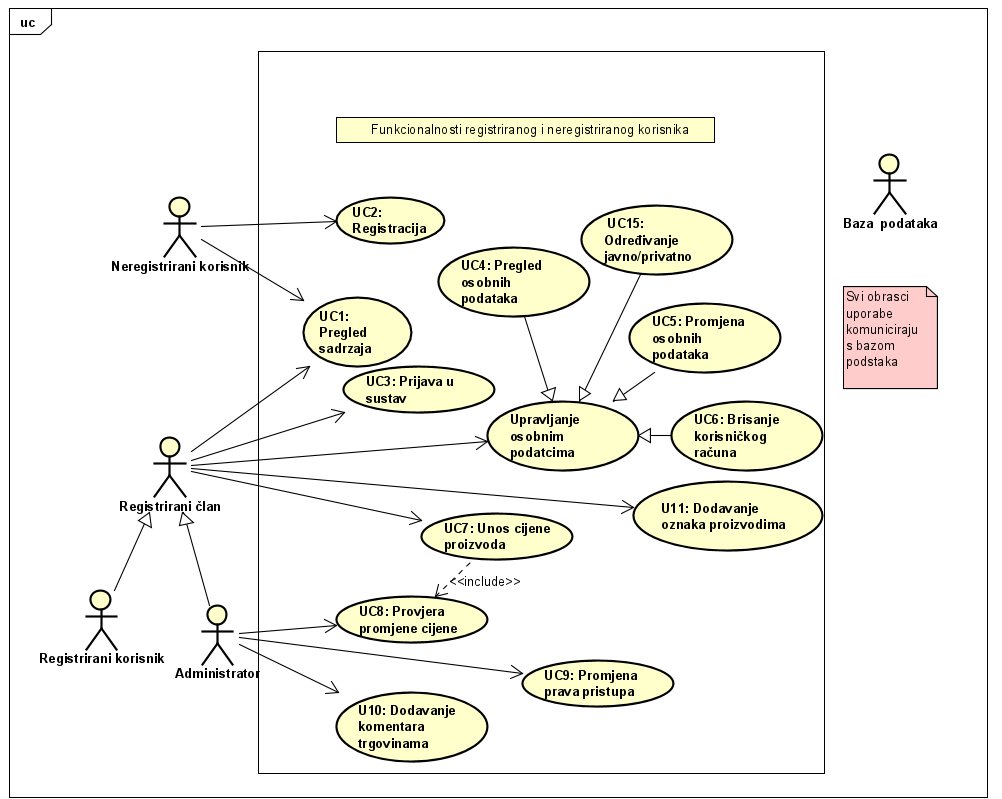
\includegraphics[width=\textwidth]{slike/Korisnik.PNG} %veličina u odnosu na širinu linije
			\caption{Use case dijagram - Korisnik}
			\label{fig:Korisnik} %label mora biti drugaciji za svaku sliku
			\end{figure}
			
			\begin{figure}[H]
			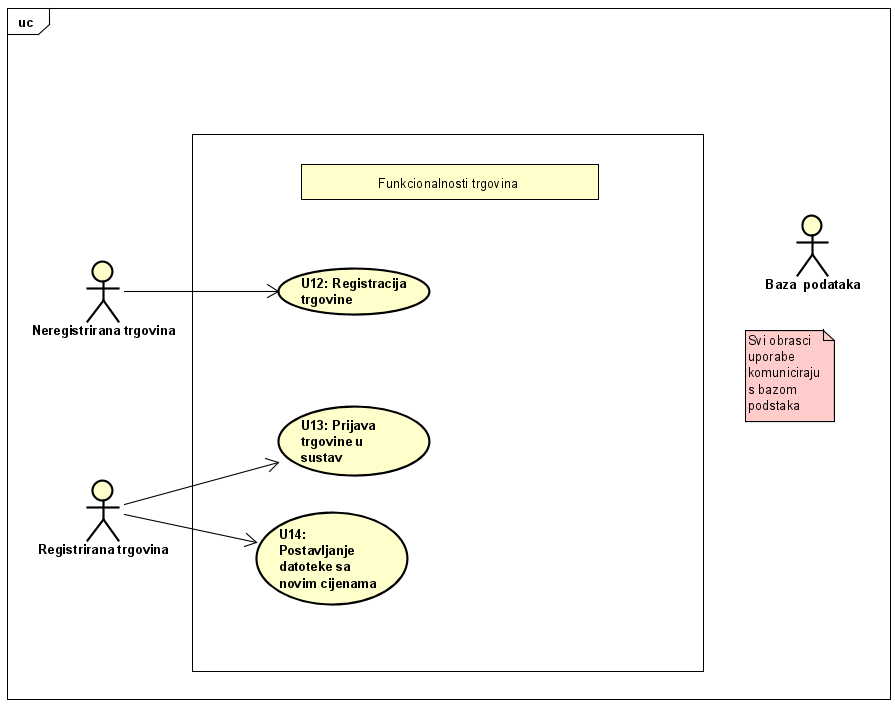
\includegraphics[width=\textwidth]{slike/Trgovina.PNG} %veličina u odnosu na širinu linije
			\caption{Use case dijagram - Trgovina}
			\label{fig:Trgovina} %label mora biti drugaciji za svaku sliku
			\end{figure}
				\eject		
				
			\subsection{Sekvencijski dijagrami}
				
				\textbf{\textit{dio 1. revizije}}\\
				
				%\textit{Nacrtati sekvencijske dijagrame koji modeliraju najvažnije dijelove sustava (max. 4 dijagrama). Ukoliko postoji nedoumica oko odabira, razjasniti s asistentom. Uz svaki dijagram napisati detaljni opis dijagrama.}
				\underline{\textbf{UC2 - Registracija}}\\
				
				Neregistrirani korisnik želi se registrirati kako bi dobio pogodnosti registriranog korisnika. Kako bi to učinio prvu odabire opciju za registraciju nakon koje mu se pokazuje register page. Unosi korisničke podatke u predviđena polja (e-mail, korisničko ime, ime, prezime i lozinku.) Aplikacija zatim provjerava s bazom postoje li profili s tom e-mail adresom ili tim korisničkim imenom. Ako su e-mail i/ili korisničko ime zauzeti, aplikacija dojavljuje pogrešku, vraća ga na stranicu za registraciju te prikazuje obavijest da izabere neku drugu e-mail adresu ili korisničko ime. Korisnik može isprobavati slobodne opcije sve dok jedna kombinacija ne bude jedinstvena ili može odustati od registracije. Kada korisnik unese jedinstvenu kombinaciju e-maila i korisničkog imena, uspješno se registrira i sustav mu šalje obavijest o uspješnoj registraciji.
				
			\begin{figure}[H]
			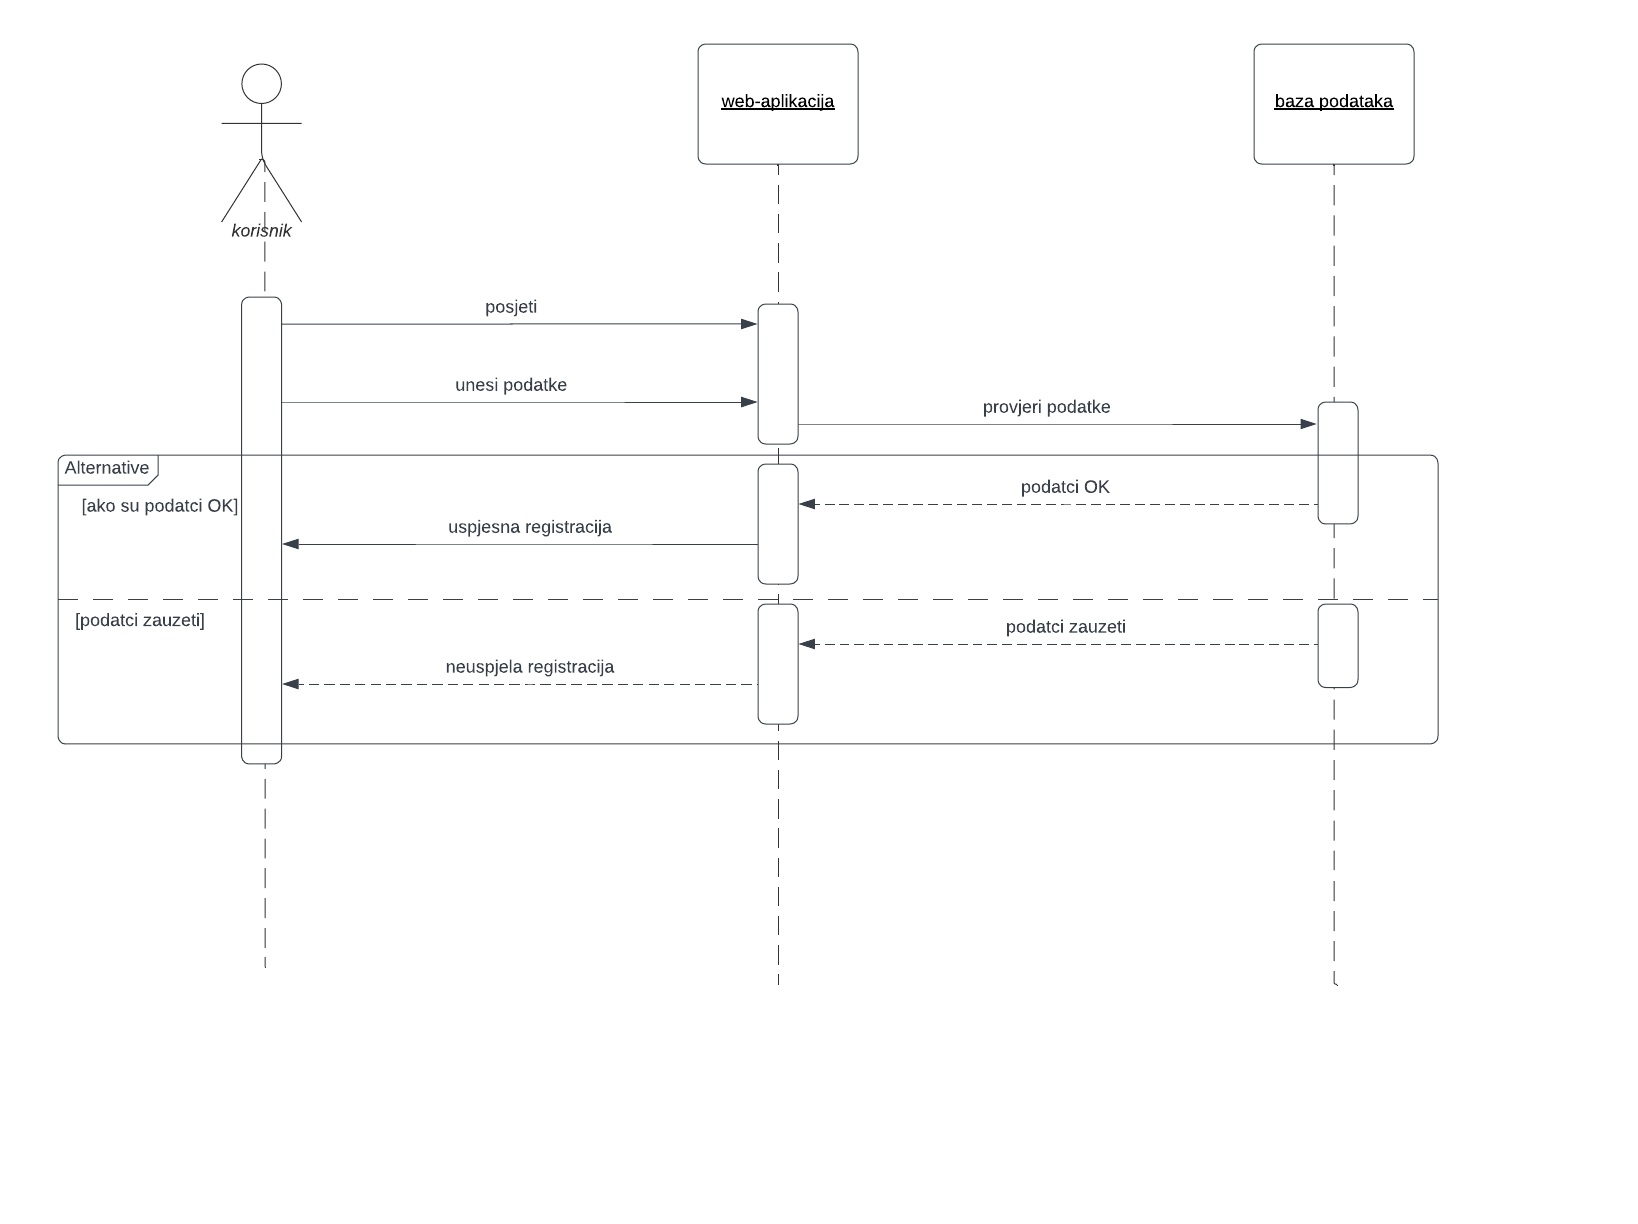
\includegraphics[width=\textwidth]{slike/uc2.PNG} %veličina u odnosu na širinu linije
			\caption{UC2 - sekvencijski dijagram}
			\label{fig:promjene2} %label mora biti drugaciji za svaku sliku
			\end{figure}
				
				\underline{\textbf{UC7 - Unos cijene proizvoda, UC8 - Provjera promjene cijene}}\\
				
				Ako postoji razlika u cijenama u trgovini i na web-stranici, korisnik odabire trgovinu u kojoj je zapazio drugačiju cijenu, unosi novu cijenu, šalje sliku proizvoda i stvarne cijene u aplikaciju. Aplikacija tu sliku sprema u bazu podataka odakle administrator odabire opciju za pregled zahtjeva, odabire zahtjev te preuzima sliku na pregled. Ako su slike u redu, administrator šalje potvrdu, cijena se promijeni te se pošalje poruka potvrde korisniku i trgovini. Ako se cijene ne podudaraju ili je zahtjev neispravan, administrator odbija zahtjev i sustav šalje obavijest korisniku o neuspjeloj promjeni cijene.
				
				\begin{figure}[H]
			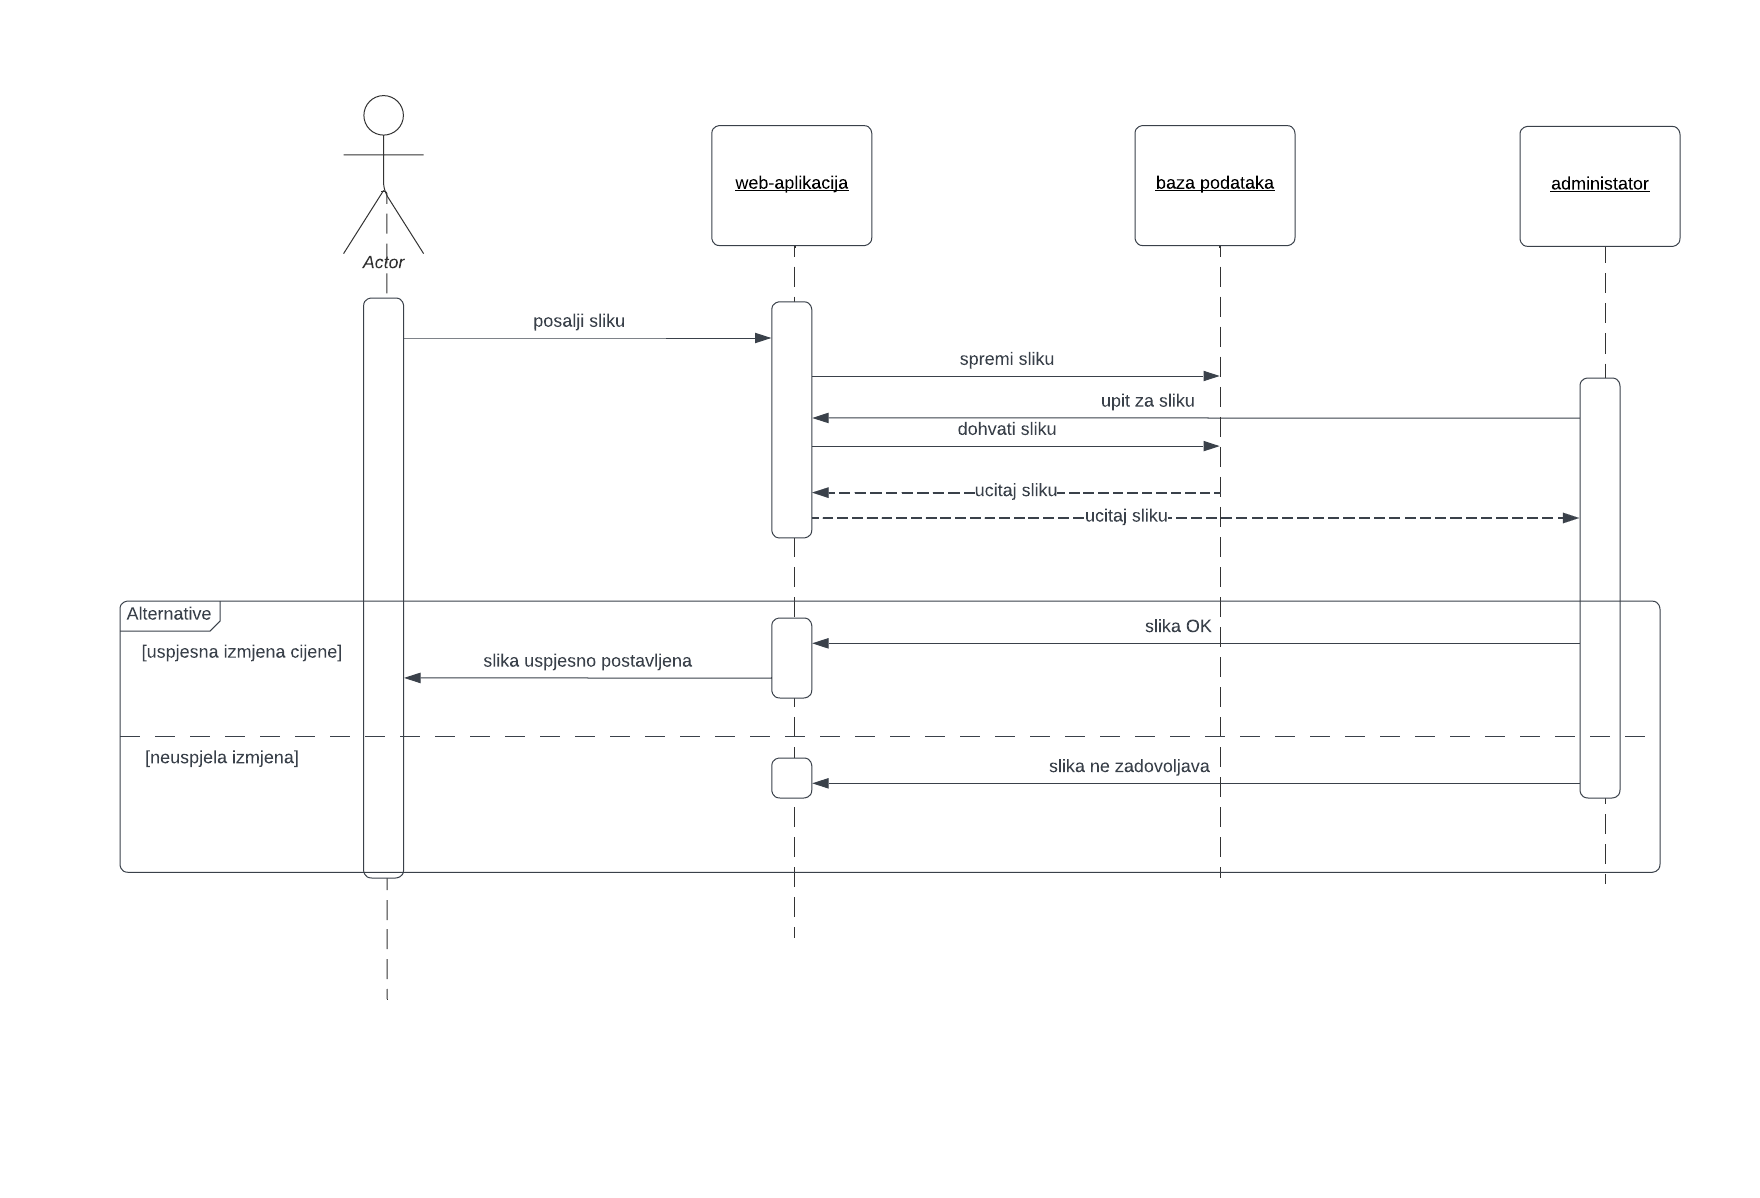
\includegraphics[width=\textwidth]{slike/uc7_cropped.PNG} %veličina u odnosu na širinu linije
			\caption{UC7, UC8 - sekvencijski dijagram}
			\label{fig:promjene2} %label mora biti drugaciji za svaku sliku
			\end{figure}
			
			\underline{\textbf{UC14 - Postavljanje datoteke sa novim cijenama}}\\
				
				Početkom svakog radnog dana trgovina unosi datoteku s promjenama cijena na svoje računalo. Web-aplikacija automatski preuzima tu datoteku i ažurira cijene u bazi podataka. Ako trgovina nije postavila datoteku, podrazumijeva se da nema promjena. Ako trgovina neispravno postavi datoteku, sustav obavještava trgovinu o neuspjeloj predaji.
				
				\begin{figure}[H]
			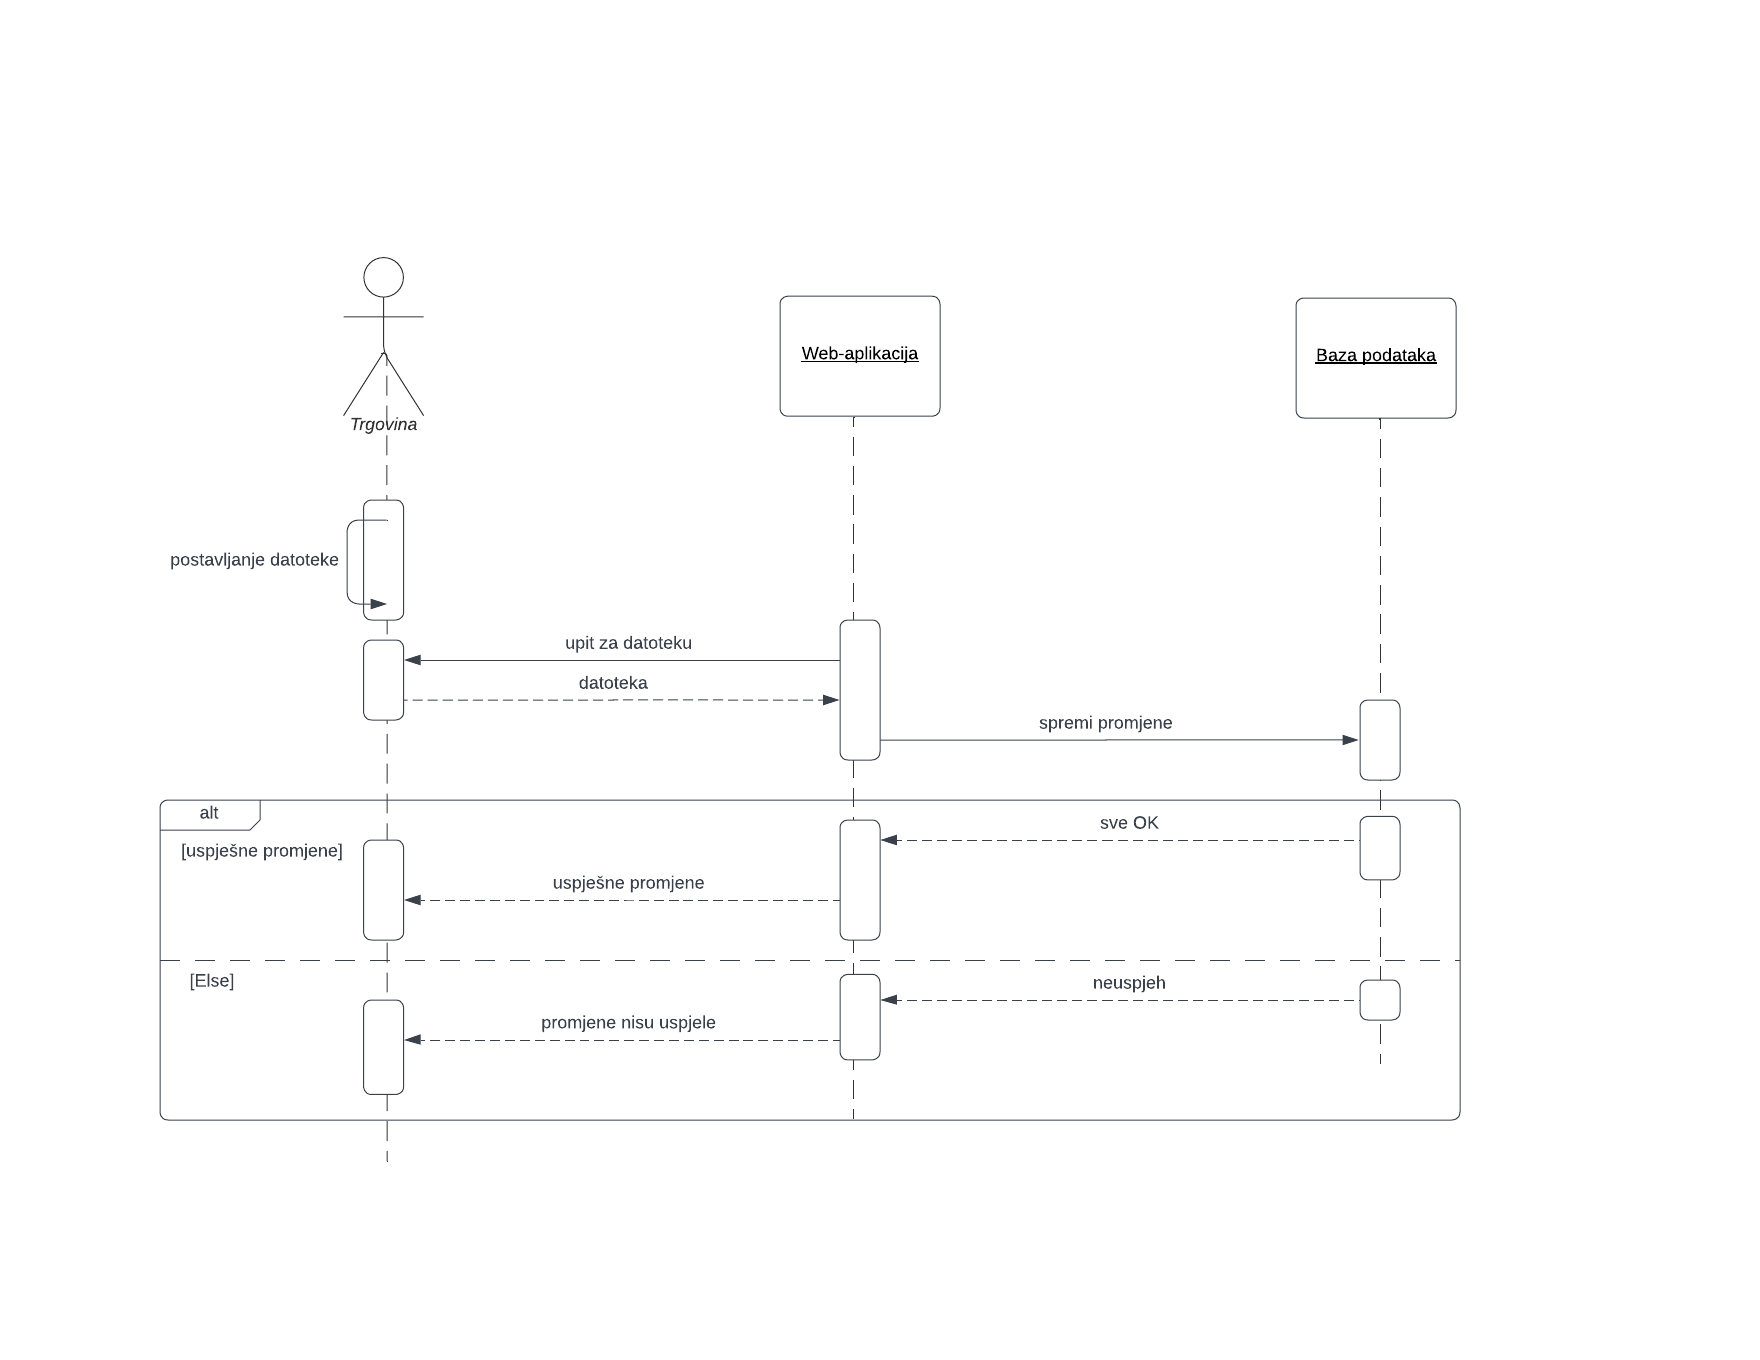
\includegraphics[width=\textwidth]{slike/uc14.PNG} %veličina u odnosu na širinu linije
			\caption{UC14 - sekvencijski dijagram}
			\label{fig:promjene2} %label mora biti drugaciji za svaku sliku
			\end{figure}
				\eject
	
		\section{Ostali zahtjevi}
		
			\textbf{\textit{dio 1. revizije}}\\
		 
			 \textit{Nefunkcionalni zahtjevi i zahtjevi domene primjene dopunjuju funkcionalne zahtjeve. Oni opisuju \textbf{kako se sustav treba ponašati} i koja \textbf{ograničenja} treba poštivati (performanse, korisničko iskustvo, pouzdanost, standardi kvalitete, sigurnost...). Primjeri takvih zahtjeva u Vašem projektu mogu biti: podržani jezici korisničkog sučelja, vrijeme odziva, najveći mogući podržani broj korisnika, podržane web/mobilne platforme, razina zaštite (protokoli komunikacije, kriptiranje...)... Svaki takav zahtjev potrebno je navesti u jednoj ili dvije rečenice.}
			 
			 
		